% CareGrid - Phase 1 Synopsis
% Complete LaTeX document with system architecture diagram
% Compile with pdfLaTeX

\documentclass[11pt,a4paper]{article}

\usepackage[a4paper,left=2.0cm,right=2.0cm,top=1.55cm,bottom=1.55cm]{geometry}
\usepackage[T1]{fontenc}
\usepackage{lmodern}
\usepackage{graphicx}
\usepackage{xcolor}
\usepackage{array}
\usepackage{tabularx}
\usepackage{ragged2e}
\usepackage{enumitem}
\usepackage{fancyhdr}
\usepackage{tikz}
\usepackage{setspace}

\usetikzlibrary{positioning,arrows.meta,shapes.geometric,fit}

% -------------------------------------------------
% COLOURS
% -------------------------------------------------
\definecolor{TitleBlue}{RGB}{61,103,154}
\definecolor{ArchitectureBlue}{RGB}{220,232,245}
\definecolor{ArchitectureGreen}{RGB}{225,240,225}
\definecolor{ArchitectureYellow}{RGB}{248,240,210}
\definecolor{ArchitectureGray}{RGB}{238,238,238}

% -------------------------------------------------
% GENERAL SETTINGS
% -------------------------------------------------
\setlength{\parindent}{0pt}
\setlength{\parskip}{0pt}
\renewcommand{\arraystretch}{1.0}

\newcommand{\blueheading}[1]{%
    {\sffamily\color{TitleBlue}\fontsize{15}{18}\selectfont #1}%
}

\newcommand{\bluebigheading}[1]{%
    {\sffamily\bfseries\color{TitleBlue}\fontsize{16}{19}\selectfont #1}%
}

\newcommand{\instruction}[1]{%
    {\itshape\fontsize{10.5}{12.5}\selectfont #1}%
}

\newcommand{\answerbox}[2][3.0cm]{%
    \vspace{2pt}
    \noindent
    \fbox{%
        \begin{minipage}[t][#1][t]{\dimexpr\textwidth-2\fboxsep-2\fboxrule\relax}
            \vspace{1mm}
            \itshape #2
        \end{minipage}
    }
}

% -------------------------------------------------
% HEADER / FOOTER
% -------------------------------------------------
\pagestyle{fancy}
\fancyhf{}
\renewcommand{\headrulewidth}{0pt}
\renewcommand{\footrulewidth}{0pt}

\fancyhead[L]{%
    \sffamily\bfseries\itshape\fontsize{10.5}{12}\selectfont
    B.TECH OSDBMS-V-2026-T219
}

\fancyhead[R]{%
    \sffamily\bfseries\fontsize{10.5}{12}\selectfont
    PROJECT PROPOSAL
}

\fancyfoot[R]{%
    \itshape\fontsize{10}{12}\selectfont
    Page \thepage
}

\setlength{\headheight}{14pt}
\setlength{\headsep}{23pt}
\setlength{\footskip}{24pt}

% -------------------------------------------------
% DOCUMENT
% -------------------------------------------------
\begin{document}

% =================================================
% PAGE 1
% =================================================

\vspace*{4mm}

\bluebigheading{PROJECT AND TEAM INFORMATION}

\vspace{13mm}

\blueheading{Project Title}

\vspace{1mm}

\answerbox[1.0cm]{CareGrid: Hospital Management and Resource Coordination System}

\vspace{13mm}

\blueheading{Student / Team Information}

\vspace{2mm}

\noindent
\begin{tabularx}{\textwidth}
{|>{\RaggedRight\arraybackslash}p{0.55\textwidth}|
 >{\RaggedRight\arraybackslash}X|}
\hline

\begin{minipage}[t]{\linewidth}
\vspace{1.5mm}
\textit{Team Name:}\\[-1mm]
\textit{Team \#}
\vspace{1.5mm}
\end{minipage}
&
\begin{minipage}[t]{\linewidth}
\vspace{1.5mm}
\textit{Avengers}
\vspace{1.5mm}
\end{minipage}
\\
\hline

\begin{minipage}[t][3.25cm][t]{\linewidth}
\vspace{1.5mm}
\textbf{Team member 1 (Team Lead)}\\[-1mm]
\textit{(Last Name, name: student ID: email, picture):}
\vspace{2.0cm}
\end{minipage}
&
\begin{minipage}[t][3.25cm][t]{\linewidth}
\vspace{1.5mm}
\textit{Singh, Mayank-240212146}\\
\textit{mayanksingh24062006@gmail.com}

\vspace{2mm}
\includegraphics[
width=2.5cm,
height=1.8cm,
keepaspectratio
]{mayank.jpeg}
\end{minipage}
\\
\hline

\begin{minipage}[t][3.25cm][t]{\linewidth}
\vspace{1.5mm}
\textbf{Team member 2}\\[-1mm]
\textit{(Last Name, name: student ID: email, picture):}
\vspace{2.0cm}
\end{minipage}
&
\begin{minipage}[t][3.25cm][t]{\linewidth}
\vspace{1.5mm}
\textit{Negi, Akshita-240221861}\\
\textit{akshitanegi0106@gmail.com}

\vspace{2mm}
\includegraphics[
width=2.5cm,
height=1.8cm,
keepaspectratio
]{Report/akshitaimg (1).jpeg}
\end{minipage}
\\
\hline

\begin{minipage}[t][3.25cm][t]{\linewidth}
\vspace{1.5mm}
\textbf{Team member 3}\\[-1mm]
\textit{(Last Name, name: student ID: email, picture):}
\vspace{2.0cm}
\end{minipage}
&
\begin{minipage}[t][3.25cm][t]{\linewidth}
\vspace{1.5mm}
\textit{Uniyal, Tanishtha-24022512}\\
\textit{tanishthauniyal30@gmail.com}

\vspace{2mm}
\includegraphics[
width=2.5cm,
height=1.8cm,
keepaspectratio
]{tanishtha.JPG}
\end{minipage}
\\
\hline

\end{tabularx}

\newpage

% =================================================
% PAGE 2
% =================================================

\bluebigheading{PROPOSAL DESCRIPTION }

\vspace{12mm}

\blueheading{Motivation }

\vspace{1mm}

\answerbox[3.0cm]{%
Hospitals manage many activities at the same time, such as patient registration, appointments, bed allocation and billing. When several users access the same resource, conflicts can occur. For example, two users may try to assign the same ICU bed. Our system provides one platform to manage hospital information and resources. OS concepts such as threads and synchronization will handle simultaneous requests, while the DBMS will keep the data accurate and organized.
}

\vspace{12mm}

\blueheading{State of the Art / Current solution }

\vspace{1mm}

\answerbox[3.5cm]{%
Hospitals commonly use Hospital Management Systems to manage patients, appointments, doctors, beds, billing and medical records. These systems handle the regular operations of a hospital, but managing shared resources when multiple requests occur at the same time can still be challenging. For example, two users may try to book the same bed or appointment slot. Our system addresses this problem by using OS synchronization techniques such as threads and mutexes, along with DBMS transactions, to ensure that resources are allocated safely and the stored information remains consistent.
}

\vspace{12mm}

\blueheading{Project Goals and Milestones }

\vspace{1mm}

\answerbox[4.15cm]{%
The main goal is to develop a Hospital Management System for managing patients, doctors, appointments and hospital resources.

Initial milestones:
\begin{itemize}[leftmargin=*,itemsep=1pt]
\item Design the system and database.
\item Develop patient, doctor and appointment modules.
\item Add bed/resource allocation with OS synchronization.
\item Test database operations and simultaneous requests.
\end{itemize}
}

\vspace{12mm}

\blueheading{Project Approach }

\vspace{1mm}

\answerbox[3.5cm]{%
The system will be developed as a web application using Python with Flask for the backend and MySQL or PostgreSQL for storing and managing data. Doctors, receptionists, hospital staff, and administrators will access the system according to their roles. The central health hub will receive requests and check the latest hospital resource information. OS concepts such as processes, threads, mutexes, and semaphores will be used to handle concurrent requests and prevent conflicts during resource allocation. DBMS concepts such as SQL, keys, constraints, and transactions will be used to maintain accurate and consistent records.
}

\newpage

% =================================================
% PAGE 3
% SYSTEM ARCHITECTURE
% =================================================

\blueheading{System Architecture (High Level Diagram)}

\vspace{5mm}

\answerbox[12.0cm]{%

\centering
\begin{tikzpicture}[
    node distance=7mm and 9mm,
    box/.style={
        draw,
        rounded corners=2pt,
        align=center,
        minimum width=3.2cm,
        minimum height=0.9cm,
        font=\sffamily\small
    },
    userbox/.style={
        box,
        fill=ArchitectureGray
    },
    backend/.style={
        box,
        fill=ArchitectureBlue,
        minimum width=4.0cm,
        minimum height=1.0cm
    },
    osbox/.style={
        box,
        fill=ArchitectureYellow,
        minimum width=4.0cm
    },
    dbbox/.style={
        box,
        fill=ArchitectureGreen,
        minimum width=4.0cm
    },
    hospital/.style={
        draw,
        rounded corners=3pt,
        align=center,
        minimum width=3.0cm,
        minimum height=1.0cm,
        fill=ArchitectureGray,
        font=\sffamily\small
    },
    arrow/.style={
        -{Latex[length=2mm]},
        thick
    }
]

% ---------------- USER LAYER ----------------

\node[userbox] (admin)
{Central Administrator};

\node[userbox, right=of admin] (staff)
{Hospital Staff};

\node[userbox, right=of staff] (users)
{Patients / Doctors};

% ---------------- CENTRAL HUB ----------------

\node[backend, below=12mm of staff] (web)
{CareGrid Web Application\\
Python + Flask};

\node[osbox, below=8mm of web] (os)
{OS Concurrency Layer\\
Processes / Threads\\
Mutexes / Semaphores};

\node[dbbox, below=8mm of os] (db)
{Central Relational Database\\
MySQL / PostgreSQL\\
Patients -- Doctors -- Appointments\\
Beds -- Resources -- Billing};

% ---------------- HOSPITALS ----------------

\node[hospital, below left=16mm and 10mm of db] (h1)
{Hospital 1\\
Beds / Doctors / Machines};

\node[hospital, below=16mm of db] (h2)
{Hospital 2\\
Beds / Doctors / Machines};

\node[hospital, below right=16mm and 10mm of db] (h3)
{Hospital N\\
Beds / Doctors / Machines};

% ---------------- USER CONNECTIONS ----------------

\draw[arrow] (admin) -- (web);
\draw[arrow] (staff) -- (web);
\draw[arrow] (users) -- (web);

% ---------------- INTERNAL FLOW ----------------

\draw[arrow] (web) -- node[right,font=\scriptsize]
{Requests} (os);

\draw[arrow] (os) -- node[right,font=\scriptsize]
{Safe concurrent access} (db);

% ---------------- HOSPITAL CONNECTIONS ----------------

\draw[arrow] (db) -- node[left,font=\scriptsize]
{Resource status} (h1);

\draw[arrow] (db) -- node[right,font=\scriptsize]
{Resource status} (h2);

\draw[arrow] (db) -- node[right,font=\scriptsize]
{Resource status} (h3);

% ---------------- RETURN FLOW ----------------

\draw[arrow] (h1) -- node[left,font=\scriptsize]
{} (db);

\draw[arrow] (h2) -- node[left,font=\scriptsize]
{Update} (db);

\draw[arrow] (h3) -- node[right,font=\scriptsize]
{} (db);

\end{tikzpicture}

}

\vspace{10mm}

\blueheading{Project Outcome / Deliverables }

\vspace{1mm}

\answerbox[7cm]{%
The project will deliver a working Hospital Management and Resource Coordination System that integrates patient registration, doctor management, appointment scheduling, bed allocation, billing, and hospital resource monitoring on a unified platform. The system will maintain structured and consistent hospital information using a relational database and support concurrent requests from multiple users. Operating System concepts such as processes, threads, synchronization, mutexes, and semaphores will be used to manage simultaneous operations and prevent conflicts during resource allocation. DBMS concepts including SQL queries, transactions, constraints, and data integrity will ensure that hospital records remain accurate and consistent. The system will also enable the central hub to monitor resource availability across participating hospitals, helping in efficient coordination and allocation of beds, doctors, and other resources.

}
\newpage

\vspace{10mm}

\blueheading{Assumptions}

\vspace{3mm}

\answerbox[3.1cm]{%
The system assumes that all participating hospitals are registered on the CareGrid platform and regularly update their resource information, such as beds, doctors, and medical equipment. The project will use sample hospital and patient data for testing instead of real patient records. Different users, including hospital staff and administrators, will have role-based access to the system. This project is developed for academic purposes and is intended to support healthcare resource coordination, not to replace medical decisions or emergency services.
}



% =================================================
% PAGE 4
% REFERENCES
% =================================================

\blueheading{References}

\vspace{1mm}

\answerbox[2.65cm]{%
\begin{itemize}[leftmargin=*,itemsep=2pt]
\item GeeksforGeeks, \textit{Operating System Concepts}.
\item Silberschatz, A., Galvin, P. B.,, \textit{Operating System Concepts}.
\item GeeksforGeeks, \textit{Fundamentals of Database Systems}.
\item Python and Flask Documentation.
\end{itemize}
}

\end{document}